%%%%%%%%%%%%%%%%%%%%%%%%%%%%%%%%%%%%%%%%%%%%%%%%%%%%%%%%%%%%%%%%%%%%%%%%%%%%%%%%
% DOCUMENT SPECIFICATION
%%%%%%%%%%%%%%%%%%%%%%%%%%%%%%%%%%%%%%%%%%%%%%%%%%%%%%%%%%%%%%%%%%%%%%%%%%%%%%%%
% \documentclass[twoside,a4paper]{scrartcl}        % Koma-script class
\documentclass[a4paper]{scrartcl}               % Koma-script class

%----------------------------------------------------------------------------------------
% PREAMBLE: PACKAGES AND CONFIGURATIONS
%----------------------------------------------------------------------------------------
\input{preamble}

%----------------------------------------------------------------------------------------
% PROJECT INFORMATION: MODIFY THIS SECTION!
%----------------------------------------------------------------------------------------
\projecttitle{Deep Learning for Biodiversity Monitoring: Automated Classification of Small Mammals Captured in Foto Trap Boxes}
\projecttype{Bachelor Thesis} % Bachelor Thesis, Master Thesis, Project Report, etc.
\projectcode{}
\projectdate{\today}
\keywords{
    Camera Trapping,
    Deep Learning,
    Transfer Learning,
    Object Detection,
    Image Classification,
    Small Mammals,
    Biodiversity Monitoring,
    MegaDetector
    }

%----------------------------------------------------------------------------------------
% AUTHORS AND AFFILIATIONS
%----------------------------------------------------------------------------------------
\addauthor{A}{Julian}{Kraft}{kraftjul@students.zhaw.ch}{1}

\addcollaborator{A}{Dr. Stefan}{Glüge}{glue@zhaw.ch}{2}
\addcollaborator{B}{Dr. Matthias}{Nyfeler}{nyfe@zhaw.ch}{2}

\addaffiliation{1}
{ZHAW - Institute of Natural Resource Sciences}
{https://www.zhaw.ch/en/lsfm/institutes-centres/iunr/}
{Grüentalstrasse 14, Wädenswil, Switzerland}

\addaffiliation{2}
{ZHAW - Institute of Computational Life Sciences}
{https://www.zhaw.ch/en/lsfm/institutes-centres/icls/}
{Schloss, Wädenswil, Switzerland}


\pdfautorstring{Julian Kraft}
\university{Zurich University of Applied Sciences}
\department{Life Sciences and Facility Management}
\institute{Institute of Natural Resource Sciences} 
\group{} 

\AtBeginDocument{
\hypersetup{pdftitle=\projecttitle} % Set the PDF's title to your title
\hypersetup{pdfauthor=\pdfautorstring} % Set the PDF's author to your name
\hypersetup{pdfkeywords=\keywords} % Set the PDF's keywords to your keywords
}

%----------------------------------------------------------------------------------------
% References
%----------------------------------------------------------------------------------------
\usepackage[
    backend=biber,             % Use biber backend (an external tool)
    sorting=nyt,               % Sort by name, year, title
    style=apa,                 % Choose here your preferred citation style
    uniquename=false,          % Avoids creating unique author lists
    uniquelist=false           % Avoids creating unique author lists
]{biblatex}

\addbibresource{./biblatex_ba.bib} % The filename of the bibliography

%----------------------------------------------------------------------------------------
% Acronyms
%----------------------------------------------------------------------------------------
\acsetup{
    list/heading = section*, 
    list/name = {List of Abbreviations}
    }

% Indicate the main file. Must go at the beginning of the file.
% !TEX root = ../main.tex

\DeclareAcronym{AI}{
    short = AI,
    long  = Artificial Intelligence,
    first-style = short
}
\DeclareAcronym{BA}{
    short = BalAcc,
    long = balanced accuracy,
}
\DeclareAcronym{BBox}{
    short = BBox,
    long = bounding box,
    short-plural = es,
    long-plural = es
}
\DeclareAcronym{CNN}{
    short = CNN,
    long  = Convolutional Neural Network
}
\DeclareAcronym{CM}{
    short = CM,
    long  = confusion matrix
}
\DeclareAcronym{CSV}{
    short = CSV,
    long  = Comma-Separated Values,
    first-style = short
}
\DeclareAcronym{DL}{
    short = DL,
    long  = Deep Learning
}
\DeclareAcronym{EXIF}{
    short = EXIF,
    long  = Exchangeable Image File Format,
    first-style = short
}
\DeclareAcronym{eDNA}{
    short = eDNA,
    long  = environmental DNA
}
\DeclareAcronym{GB}{
    short = GB,
    long  = Giga Byte,
    first-style = short
}
\DeclareAcronym{GPU}{
    short = GPU,
    long  = Graphics Processing Unit,
    first-style = short
}
\DeclareAcronym{HPC}{
    short = HPC,
    long  = High Performance Computing,
    first-style = short
}
\DeclareAcronym{IUNR}{
    short = IUNR,
    long  = Institute of Natural Resource Sciences,
    first-style = short
}
\DeclareAcronym{MD}{
    short = MD,
    long  = MegaDetector
}
\DeclareAcronym{MLWIC2}{
    short = MLWIC2,
    long  = Machine Learning for Wildlife Image Classification 2
}
\DeclareAcronym{OCR}{
    short = OCR,
    long  = Optical Character Recognition
}
\DeclareAcronym{ROI}{
    short = ROI,
    long = region of interest
}
\DeclareAcronym{ViT}{
    short = ViT,
    long  = Vision Transformer
}
\DeclareAcronym{WI}{
    short = WI,
    long  = Wildlife Insights
}
\DeclareAcronym{ZHAW}{
    short = ZHAW,
    long  = Zurich University of Applied Sciences,
    first-style = short
}
 % Load the acronyms file

%----------------------------------------------------------------------------------------
% Beginning of the document
%----------------------------------------------------------------------------------------
\begin{document}
\hypersetup{linkcolor=black, urlcolor=black} % Make links black for first part

%----------------------------------------------------------------------------------------
% TITLE PAGE AND IMPRINT
%----------------------------------------------------------------------------------------
\include{front/titlepage}

%\let\cleardoublepage\clearpage % not needed for single-sided printing

\include{front/imprint}

%----------------------------------------------------------------------------------------
% handling page numbering
%----------------------------------------------------------------------------------------
\clearpage
\pagenumbering{roman}
\setcounter{page}{1}

%----------------------------------------------------------------------------------------
% ABSTRACT
%----------------------------------------------------------------------------------------
% Indicate the main file. Must go at the beginning of the file.
% !TEX root = ../main.tex

%%%%%%%%%%%%%%%%%%%%%%%%%%%%%%%%%%%%%%%%%%%%%%%%%%%%%%%%%%%%%%%%%%%%%%%%%%%%%%%%
% Abstract
%%%%%%%%%%%%%%%%%%%%%%%%%%%%%%%%%%%%%%%%%%%%%%%%%%%%%%%%%%%%%%%%%%%%%%%%%%%%%%%%

\vspace*{\fill}
\selectlanguage{english}
\section*{Abstract}
\label{abstract}

This thesis explores the use of \ac{DL} to automate the classification of small mammals captured in camera trap images gathered as part of the Wildlife@Campus project.
A dataset of over 400,000 labeled images, grouped into sequences, was processed using \ac{MD} to filter and crop relevant regions of interest.
Several model architectures were evaluated, with the pretrained EfficientNet-B0 achieving the highest balanced accuracy of \(0.992\) for the classification task.
A comprehensive data pipeline was developed, including detection, preprocessing, cross-validation and classification on an image and sequence level, enabling efficient and reproducible model training and evaluation.
While pretrained models outperformed non-pretrained variants, the results also demonstrated that smaller architectures can be accurate while saving resources.
The study highlights the feasibility of DL for small mammal classification in the given context, the importance of detection quality, label accuracy and the need for a non-target class to handle unknown species such as snails or misdetections such as plant parts or simply empty images.
In addition to the missing non-target class, the study also emphasizes the need for an improved detection process in order to reduce missed sightings.
There is still a high dependency on large amounts of labeled data, which is a real challenge when adding additional classes.
This work lays the foundation for integrating \ac{DL} into the camera trap approach of the Wildlife@Campus project, aiming to reduce the associated manual effort in small mammal monitoring and contribute to ecological research.
\vspace*{\fill}

\newpage

\vspace*{\fill}
\selectlanguage{ngerman}
\section*{Zusammenfassung}

\sloppy{Diese Bachelorarbeit untersucht den Einsatz von \ac{DL} zur automatisierten Klassifikation von Kleinsäugern, die mithilfe von Kamerafallen im Rahmen des Wildlife@Campus-Projekts erfasst wurden.}
Ein Datensatz mit über 400'000 annotierten Bildern, gruppiert in Sequenzen, wurde mithilfe von \ac{MD} verarbeitet, um relevante Bildausschnitte zu filtern und zuzuschneiden.
Mehrere Modellarchitekturen wurden evaluiert, wobei das vortrainierte EfficientNet-B0 die höchste Balanced Accuracy von \(0{,}992\) für die Klassifikationsaufgabe erzielte.
Es wurde eine umfassende Datenpipeline entwickelt, die Erkennung, Vorverarbeitung, Kreuzvalidierung sowie Klassifikation auf Bild- und Sequenzebene umfasst und ein effizientes sowie reproduzierbares Modelltraining und eine entsprechende Evaluation ermöglicht.
Während vortrainierte Modelle gegenüber nicht vortrainierten Varianten bessere Leistungen zeigten, verdeutlichten die Ergebnisse auch, dass kleinere Architekturen präzise sein können und gleichzeitig Ressourcen sparen.
Die Studie betont Anwendbarkeit von \ac{DL} für die Klassifikation von Kleinsäugern in diesem Kontext, die Bedeutung der Detektionsqualität, der Labelgenauigkeit und die Notwendigkeit einer Sonstige-Klasse zur Berücksichtigung unbekannter Arten wie z.B. Schnecken oder Fehldetektionen wie z.B. Pflanzenteile oder leere Bilder.
Neben der fehlenden Sonstige-Klasse unterstreicht die Studie auch den Bedarf nach einem verbesserten Detektionsprozess, um verpasste Sichtungen zu reduzieren.
Zudem besteht weiterhin eine hohe Abhängigkeit von grossen Mengen annotierter Daten, was eine reale Herausforderung bei der Einführung zusätzlicher Klassen darstellt.
Diese Arbeit legt das Fundament für die Integration von \ac{DL} in den Kamerafallen-Ansatz des Wildlife@Campus-Projekts, mit dem Ziel, den damit verbundenen manuellen Aufwand bei der Kleinsäugerüberwachung zu reduzieren und zur ökologischen Forschung beizutragen.
\selectlanguage{english}
\vspace*{\fill}

%----------------------------------------------------------------------------------------
% ACKNOWLEDGEMENTS
%----------------------------------------------------------------------------------------
% Indicate the main file. Must go at the beginning of the file.
% !TEX root = ../main.tex

%%%%%%%%%%%%%%%%%%%%%%%%%%%%%%%%%%%%%%%%%%%%%%%%%%%%%%%%%%%%%%%%%%%%%%%%%%%%%%%%
% Aknowledgement
%%%%%%%%%%%%%%%%%%%%%%%%%%%%%%%%%%%%%%%%%%%%%%%%%%%%%%%%%%%%%%%%%%%%%%%%%%%%%%%%

\vspace*{\fill}

\section*{Acknowledgments}
\label{acknowledgments}

I am deeply grateful to my supervisor, Dr. Stefan Glüge, for his invaluable guidance and interesting discussions throughout this thesis. 
My thanks also go to Dr. Matthias Nyfeler, who provided the topic and ensured I had all the support needed troughout the project. 
I want to thank Prof. Dr. Roland Felix Graf and Nils Ratnaweera for their help in obtaining the data and all the information I needed on the Wildlife@Campus project to get started with the thesis. 
Finally, I would like to thank the HPC-support team --- especially Dr. Pascal Häussler --- for their assistance with the cluster and their impressively swift responses to my questions.

\vspace*{\fill}


%----------------------------------------------------------------------------------------
% LIST OF CONTENTS/FIGURES/TABLES PAGES
%----------------------------------------------------------------------------------------
% Comment out if any of the following is not needed:
\tableofcontents  % Add main table of contents

\hypersetup{linkcolor=linkcolor, urlcolor=urlcolor}
\textbf{Code, and LaTeX source are to be found on GitHub:}\\
\url{https://github.com/juliankraft/BachelorThesis}
\hypersetup{linkcolor=black, urlcolor=black}

\newpage
\listoffigures    % Add list of figures
\listoftables     % Add list of tables
\printacronyms    % Add list of acronyms

\hypersetup{linkcolor=linkcolor, urlcolor=urlcolor} % Reset to default after TOC

%%%%%%%%%%%%%%%%%%%%%%%%%%%%%%%%%%%%%%%%%%%%%%%%%%%%%%%%%%%%%%%%%%%%%%%%%%%%%%%%
% THESIS CONTENT - CHAPTERS
%%%%%%%%%%%%%%%%%%%%%%%%%%%%%%%%%%%%%%%%%%%%%%%%%%%%%%%%%%%%%%%%%%%%%%%%%%%%%%%%

%----------------------------------------------------------------------------------------
% handling page numbering
%----------------------------------------------------------------------------------------
\clearpage
\pagenumbering{arabic}
\setcounter{page}{1}
%\mainmatter                     % Begin numeric (1,2,3...) page numbering
%\pagestyle{reportStyle}              % Reset the page headers

% Indicate the main file. Must go at the beginning of the file.
% !TEX root = ../main.tex

%%%%%%%%%%%%%%%%%%%%%%%%%%%%%%%%%%%%%%%%%%%%%%%%%%%%%%%%%%%%%%%%%%%%%%%%%%%%%%%%
% 01-introduction
%%%%%%%%%%%%%%%%%%%%%%%%%%%%%%%%%%%%%%%%%%%%%%%%%%%%%%%%%%%%%%%%%%%%%%%%%%%%%%%%

\section{Introduction}
\label{introduction}

The loss of biodiversity is one of the most pressing issues of our time \autocite{cardinaleBiodiversityLossIts2012}.
Agricultural expansion, urbanization, and climate change are just a few of the many factors that threaten biodiversity.
For a better understanding of the impact of these factors and the development of effective conservation strategies or simply to track what is being lost it is crucial to monitor biodiversity.
This task has traditionally been done by trained experts, who manually identify species in the field or in images.
Accessible and cheap sensors as well as improved battery and storrage technology have made it possible to deploy large numbers of sensors in the field in order to create vast amounts of images.
The use of Deep Learning (DL) methods to handle has become a standard approach.

    \subsection{Background}
    Biodiversity in Switzerland faces significant pressure due to habitat loss and declining species numbers.
    Particularly, small mammals have received comparatively less attention in conservation research and public perception, despite their crucial ecological roles.
    Of the approximately 30 species of small mammals native to Switzerland, several are threatened and depend on targeted conservation measures.
    Detecting and monitoring small mammals is inherently challenging because these animals are often nocturnal and elusive, dwelling predominantly in dense vegetation or underground burrows.
    Traditional methods for small mammal detection, such as live trapping, are time-consuming, resource-intensive, and pose risks to animal welfare.
    Recent advances in indirect detection methods, including camera traps and environmental DNA (eDNA), offer promising alternatives that are less invasive and potentially more efficient.
    Camera trap systems, specifically optimized for small mammals, generate large volumes of image data, necessitating advanced automated image classification techniques to manage and analyze the data effectively.
    However, distinguishing closely related species visually remains challenging, thereby necessitating complementary genetic identification through collected eDNA\@.
    The integration of eDNA analysis and automated image processing within modular detection systems presents a robust approach to accurately monitor small mammal populations at a broader scale.
    Thus, ongoing research and technological enhancements in both camera trap efficiency and genetic analysis methods are crucial for improving small mammal biodiversity assessments and informing conservation strategies.

    \subsection{Problem Statement}

    Breaking down the problem to be solved.

    \subsection{Related Work}

    - Overview of related work in the field

    - specifically the use of MD
    The Microsoft MegaDetector (MD) is a well-established model for detecting animals in camera trap images \autocite{hernandezPytorchWildlifeCollaborativeDeep2024, velezChoosingAppropriatePlatform2022, schneiderRecognitionEuropeanMammals2024}.


% Indicate the main file. Must go at the beginning of the file.
% !TEX root = ../main.tex

%%%%%%%%%%%%%%%%%%%%%%%%%%%%%%%%%%%%%%%%%%%%%%%%%%%%%%%%%%%%%%%%%%%%%%%%%%%%%%%%
% 03_methods
%%%%%%%%%%%%%%%%%%%%%%%%%%%%%%%%%%%%%%%%%%%%%%%%%%%%%%%%%%%%%%%%%%%%%%%%%%%%%%%%

\section{Methods}
\label{methods}

    \subsection{Dataset}

    As part of the Wildlife@Campus project, a labeled dataset was created to train a deep learning algorithm.
    This dataset is divided into seven sessions -- indicating the project stage where the data was added to the dataset.
    The images are grouped into sequences, each sequence representing a sightin of an animal.
    Somehow the sequences are not standardized in length and range from 1 to 915 images per sequence.
    It is worth noting that in future use cases, the sequence length will likely be more standardized.
    The actual length will depend on the camera settings -- common settings such as 1, 3, 5, or 10 images per trigger -- which can be extracted from the EXIF information of the images.
    For this project, the sequences will be used as they are, and the length will not be standardized.
    The dataset provides two types of labels: the first one is not yet standardized troughout the sessions and contains a variety of labels for the same species.
    For example scientific names and common names are used interchangeably, and there are different spellings.
    The second type is a simplified and standardized version with some visually not distinguishable species grouped together.
    For this project, only the simplified labels will be used.
    To get an overview of the available sequences per label, refere to \autoref{fig:sequenceperlabel}.
    The category \texttt{other} represents sequences containing more than one species, this is a result of the process creating the sequences.
    Furthermore the category \texttt{NaN} represents sequences not labeled -- both will be excluded from the from the dataset.
    The category \texttt{glis\_glis} is represented in only four sequences, which is simply not enough to actually train the model to detect it.
    For this reason, it will be excluded from the dataset as well.
    This leaves four categories for the classification task: \texttt{apodemus\_sp}, \texttt{cricetidae}, \texttt{soricidae}, and \texttt{mustela\_erminea}.

    \begin{figure}[ht]
    \centering
    \includegraphics{figures/label2_session.pdf}
    \caption{Available sequences per label colored by session.}
    \label{fig:sequenceperlabel}
    \end{figure}

    \subsection{Data Processing}

    The processing of the images is divided into two main steps: 
    In a first step a detector is applied to identify the regions of interest (ROI) for the images, and to select which images are actually used for training.
    In a second step, the ROIs are processed to be feed into the model.

        \subsubsection{Detection and Selection}
        
        In this project, the Megadetector (MD) \autocite{morrisEfficientPipelineCamera2025} is used to identify regions of interest (ROI) on all the images.
        The MD outputs a list of bounding boxe (BBox) for detected objects labeled \textit{animal}, \textit{human} or \textit{vehicle} with a corresponding confidence value.
        For each image only the BBox with the highest confidence score -- above a threshold of 0.5 -- for the label \textit{animal} is considered.
        The percentage of images discarded dew to this process is  shown per sequence in \autoref{fig:lost_images}.
        An example of how this detections look like is shown in \autoref{fig:detection_example}.

        \begin{figure}[ht]
        \centering
        \includegraphics{figures/discarded_img_by_conf.pdf}
        \caption{Fraction of images discarded per category for a detection confidence threshold of 0.5.}
        \label{fig:lost_images}
        \end{figure}

        \begin{figure}[ht]
        \centering
        \includegraphics{figures/detections_on_a_sequence.pdf}
        \caption{Example of how the detections look like. The bounding boxes are the six highest confidence detections for the sequence 1001824 a sample from the \textit{apodemus\_sp} category.}
        \label{fig:detection_example}
        \end{figure}

        \subsubsection{Image Processing}
        To process the images a custom transformation pipline was implemented using transform version 2 from the torchvision library and a custom crop function.
        This transformation is applied on the fly by the PyTorch DataLoader.
        Cropping was done using the BBoxes from the MD detection extending the BBox in order to cut the ratio expected by the model applied.
        In the case that the extended BBox surpasses the image border the image is padded with black pixels.
        After cropping the image is resized to the expected input size of the model.
        The images are then converted to a tensor and normalized using the mean and standard deviation calculated on the dataset itself.
        To calculate mean and standard deviation the whole dataset was used since it is quite resource intensive to calculate and the same values are used for all folds.
        To create the most accurate mean and standard deviation for the actual model input only the best BBox area per image is used.
        Data augmentation a well established way to improve model's generalization \autocite{shortenSurveyImageData2019} was implemented and considered as an option but not actually used in the end.

        \subsubsection{Data Splitting}

        The dataset is split into five folds using a stratified split based on the classes.
        A custom helper function was implemented to ensure the splits are done on a sequence level, meaning no sequence is ever split between folds, while still maintaining a balanced distribution of images across the folds.
        For each class in the dataset, all the sequences are shuffled using a fixed seed for reproducibility resulting in two lists: one with the sequence ids and one with the corresponding sequence lengths.
        To build five stratified folds, it steps through the shuffled list of sequence-lengths and chooses cut-points so that each fold's sum of images is as close as possible to one-fifth of that class's total images.
        In this way, every fold ends up with roughly the same number of images per class, and no sequence is ever split between folds.

    \subsection{Model}

    In this project, a selection of models from the torchvision library was tested to classify the images. 
    Every model was both trained from scratch and fine-tuned using the weights of a model pre-trained on ImageNet \autocite{dengImageNetLargescaleHierarchical2009}.
    A custom helper function was implemented to adapt the last layer of the model to fit the number of classes in the dataset when the model is loaded.
    The models used in this project are:

    \begin{itemize}
        \item \textbf{EfficientNet-B0} \autocite{tanEfficientNetRethinkingModel2019}:  
        A Convolutional Neural Network architecture that uses a compound scaling method to uniformly scale network width, depth, and resolution.  
        The B0 variant is the baseline model from which larger EfficientNets are derived.  

        \item \textbf{DenseNet-169} \autocite{huangDenselyConnectedConvolutional2017}:  
        A densely connected convolutional network with 169 layers in which each layer receives feature-maps from all preceding layers, fostering feature reuse and improved gradient flow.  

        \item \textbf{ResNet-50} \autocite{heDeepResidualLearning2016}:  
        A 50‐layer Residual Network that introduces skip connections (residual blocks) to alleviate the vanishing-gradient problem, enabling training of very deep models.  

        \item \textbf{ViT-B\_16} \autocite{dosovitskiyImageWorth16x162021}:  
        The “Base” Vision Transformer model which splits an image into \(16\times 16\) patches, linearly embeds them, and processes the resulting sequence with a standard Transformer encoder.  
    \end{itemize}

    \subsection{Training}

    The training process is divided into four main steps repeated for each fold of the cross-validation:
    \begin{enumerate}
        \item Loading the dataset and applying the preprocessing steps described above.
        \item Initializing the model with the appropriate architecture and adapting the last layer to match the classes.
        \item Training the model for the current fold using the training set only keeping the last and the best version of the model.
        \item The best version of the model is loaded to predict the whole dataset for later evaluation.
    \end{enumerate}

    During training, the loss is calculated using the cross-entropy loss function with the class weights calculated on the current training set.
    To adjust the model parameters, the AdamW optimizer \autocite{loshchilovDecoupledWeightDecay2019} is used with a weight decay of $10^{-5}$ and an initial learning rate of $10^{-4}$.
    The learning rate is adjusted using a cosine annealing scheduler \autocite{loshchilovSGDRStochasticGradient2017} over 50 epochs.
    A maximum of 50 epochs where trained, but an early stopping callback was implemented monitoring the validation loss with a patience of 10 epochs.
    The logging is done using the tensorboard logger, which is integrated into PyTorch Lightning and an additional custom CSV logger for easier log access for evaluation.
    A batch size of 64 was used for training -- and doubled for validation and prediction.
    Predicting the whole dataset the predicted class for each sample and the confidence scores per class where saved to a CSV file for later evaluation

    \subsection{Sequence Classification}
    Since the data is grouped into sequences and the classification is done per image, an additional step is performed to classify the sequences.
    This step is only performed after the model has been trained and the predictions for the whole dataset are available.
    To classify the sequences, the image-level predictions are aggregated by sequence ID and the confidence scores for each class are summed across all images in the sequence.
    To normalize this summed confidences, they each are divided by the total sum of all summed confidences in that sequence.
    From this normalized confidences, the class with the highest confidence is selected as the predicted class for the sequence.

    \subsection{Evaluation}

    The evaluation is done using the predictions created by the best version of every model for each fold.
    Both the image-level and sequence-level predictions are evaluated using the balanced accuracy score \autocite{brodersenBalancedAccuracyIts2010} as the main metric.
    The balanced accuracy score is calculated using the following formula:
    \begin{equation}
    \text{Balanced Accuracy}
    \;=\;
    \frac{1}{K} \sum_{c=1}^{K}
        \frac{TP_{c}}{\,TP_{c} + FN_{c}\,}
    \end{equation}

    \noindent where:
    \begin{description}
    \item[$K$] is the total number of classes.
    \item[$TP_{c}$] (true positives for class $c$) is the count of samples whose true label is $c$ and whose predicted label is also $c$.
    \item[$FN_{c}$] (false negatives for class $c$) is the count of samples whose true label is $c$ but whose predicted label is not $c$.
    \end{description}


    \subsection{Hardware and Software}

    This project was processed on the IUNR HPC cluster using node 301, an HPE Apollo 6500 Gen10+ node running Rocky Linux 8. 
    The node is equipped with 8 NVIDIA L40S GPUs (48 GB each), dual AMD EPYC 7742 processors, 512 cores, and 5800 GB of storage, providing the computational power needed for high-performance tasks.

    The software environment includes:
    
    \begin{itemize} 
        \item Python 3.10
        \item PyTorch 2.1.0
        \item PyTorch Lightning 2.5.1 \autocite{falconPyTorchLightning2025}
        \item sklearn
    \end{itemize} \todo{This list needs to be updated with the actual versions used.}

    On the GitHub repository a yaml file is provided to reproduce the environment using conda.


% Indicate the main file. Must go at the beginning of the file.
% !TEX root = ../main.tex

%%%%%%%%%%%%%%%%%%%%%%%%%%%%%%%%%%%%%%%%%%%%%%%%%%%%%%%%%%%%%%%%%%%%%%%%%%%%%%%%
% 04_results
%%%%%%%%%%%%%%%%%%%%%%%%%%%%%%%%%%%%%%%%%%%%%%%%%%%%%%%%%%%%%%%%%%%%%%%%%%%%%%%%

\section{Results}
\label{results}

    \subsection{Detection}

    - after detection how many sequences are excluded

    - how many images are left per label

    \subsection{Model Performance}

    - Table with all the models and their performance (Loss, Balanced Accuracy for the image and sequence level)

    \subsection{Best Model}

    - More information on the best model including CM
% Indicate the main file. Must go at the beginning of the file.
% !TEX root = ../main.tex

%%%%%%%%%%%%%%%%%%%%%%%%%%%%%%%%%%%%%%%%%%%%%%%%%%%%%%%%%%%%%%%%%%%%%%%%%%%%%%%%
% 04_discussion
%%%%%%%%%%%%%%%%%%%%%%%%%%%%%%%%%%%%%%%%%%%%%%%%%%%%%%%%%%%%%%%%%%%%%%%%%%%%%%%%


\section{Discussion}
\label{discussion}

\subsection{Detection}
The detection process significantly influenced the dataset composition, particularly on the sequence level for the category \textit{mustela\_erminea}.
This category experienced higher data loss, likely due to the relative size of the species --- it is much larger than the other species captured by these MammaliaBox camera traps.
This larger size may have resulted in more frequent bad shots due to the closeness to the camera or the speed at which they pass through the box --- many images showed only the tip of the animal's tail disappearing out of the box.
Another interesting observation was the fact that the white fur individuals were more often not detected than the brown fur individuals.
An explanation has yet to be found for why this was only the case on the sequence level, where the \textit{mustela\_erminea} category was disproportionately affected.
On the image level, the \textit{soricidae} category was the most affected, with \(23\%\) of the images lost but only \(1\%\) of the sequences.

Visual inspection revealed a mixture of exemplary BBox detections alongside notable inaccuracies, such as missed detections in images with obstructions or partial visibility of animals.
Looking through misclassified images with high confidence values revealed some interesting insights.
One was that quite a few false positive detections were made, leading to surprisingly high confidence classifications.
Some of these images were empty or contained no animal at all, as shown in \autoref{fig:false_positive_dt}, which includes examples where plant parts were misdetected, or possibly animals appeared in very dark areas, or some very small, not clearly visible objects.
Another interesting finding was that quite a few of the images contained a snail in the highest confidence BBox --- refer to \autoref{fig:false_class_snails} for a hand-picked selection of these examples.
These misclassifications highlight the need for enhanced object discrimination capabilities or the introduction of an additional class for non-target species.

\begin{figure}[ht]
\centering
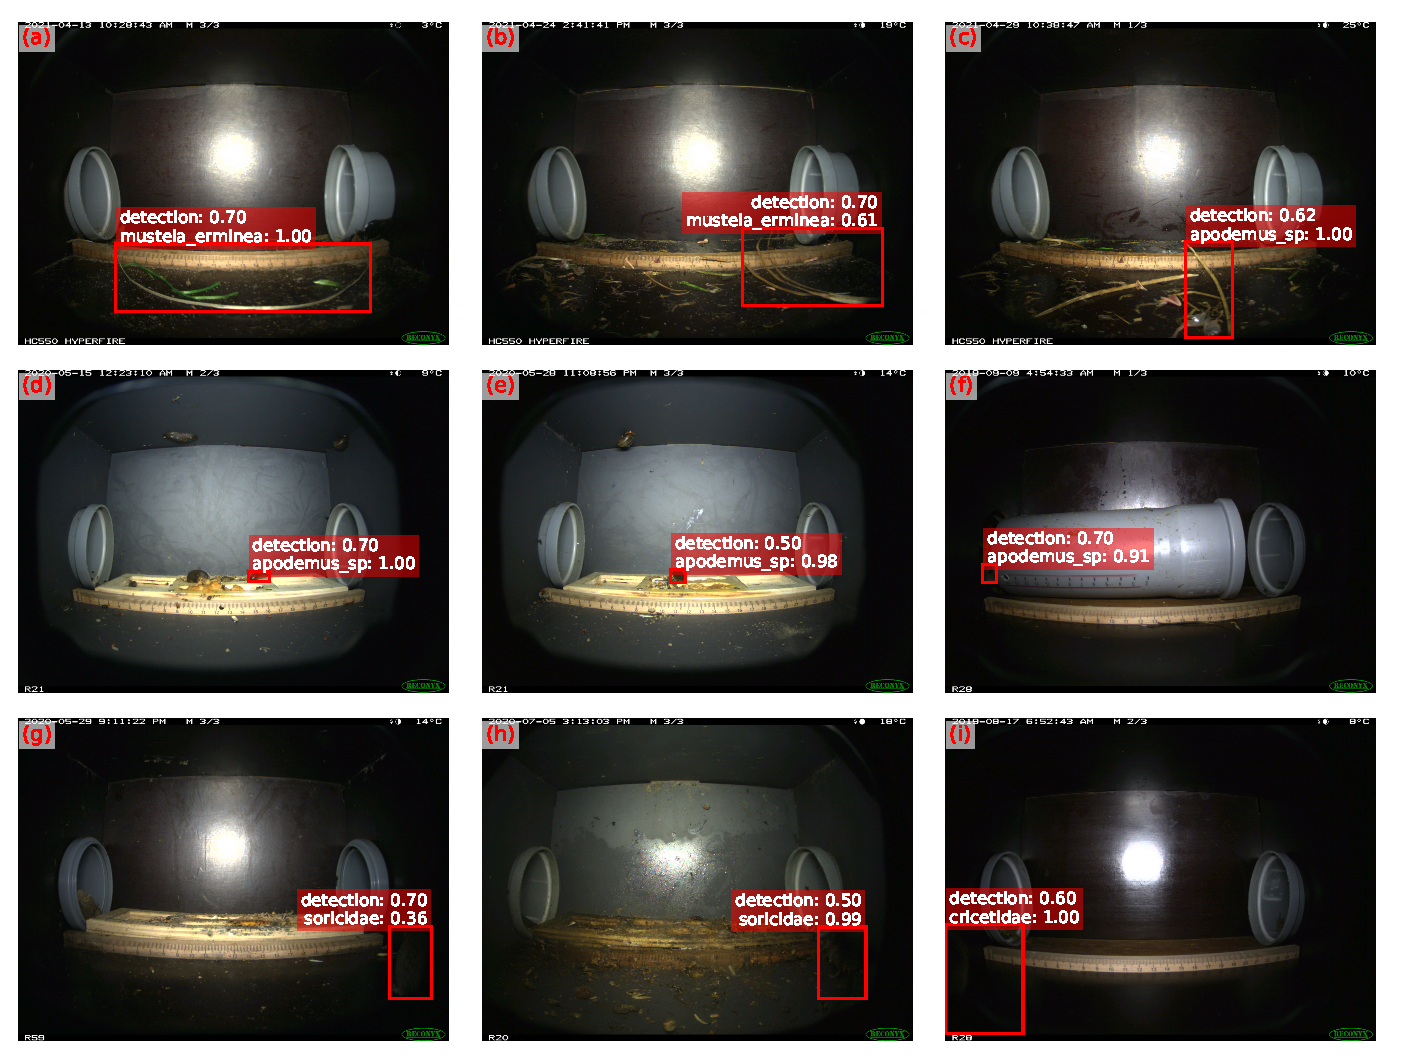
\includegraphics[width=\textwidth]{figures/false_positive_dt.pdf}
\caption{Hand-picked selection of images with a high confidence value but no animal in the image.}
\label{fig:false_positive_dt}
\end{figure}

\begin{figure}[ht]
\centering
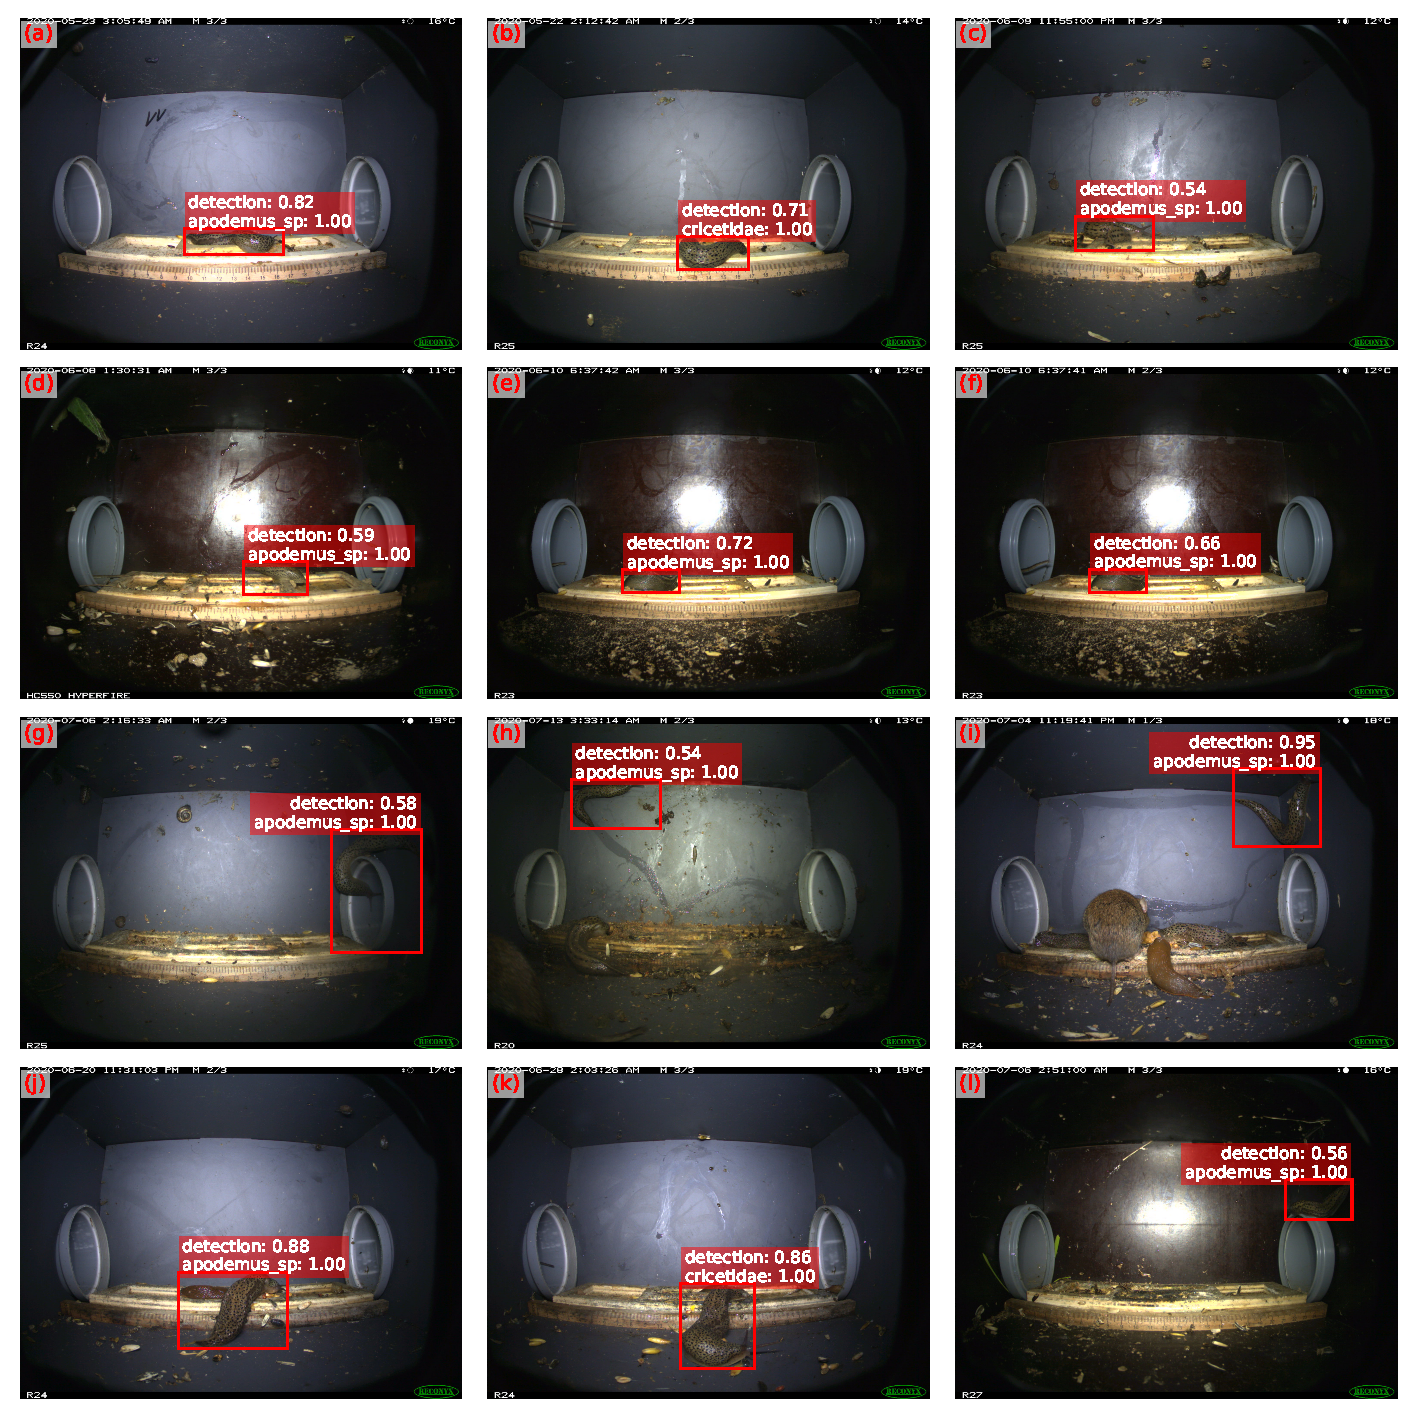
\includegraphics[width=\textwidth]{figures/false_class_snails.pdf}
\caption{Hand-picked selection of images predicted incorrectly with a high confidence value displaying a snail in the highest confidence BBox.}
\label{fig:false_class_snails}
\end{figure}

\subsection{Model Performance}
All tested models achieved high performance in image classification tasks, demonstrating their suitability for automating small mammal identification.
Pretrained models slightly outperformed those trained from scratch, underscoring the value of transfer learning.
The slightly better balanced accuracy of pretrained models is just one of the benefits of using pretrained models, as they also require less training time and computational resources and could potentially be trained with less training data.

Interestingly, the smaller the models, the better they performed on the image-level classification task, highlighting the fact that bigger is not always better.
Smaller models, if complex enough for the task, are always preferable since they require less computational resources and are faster to train.
Examining \autoref{fig:bal_acc_img} again, one could speculate about a trend for smaller models to perform more consistently across folds when trained from scratch --- but for some reason, this is not the case for the EfficientNet-B0 model.
The observations from this study suggest that smaller, computationally efficient models are sufficient and therefore preferable for the classification tasks at hand.

\subsection{Best Model Architecture}
The pretrained EfficientNet-B0 emerged as the best-performing model architecture, achieving the highest balanced accuracy.
Remarkably, the optimal validation loss was reached within the first few epochs, while \ac{BA} continued to improve \autoref{fig:training_metrics_best_model}.\todo{Why did BalAcc still improve?}
Since the training dataset was quite large, contained only four classes, and was intensively vetted using the \ac{MD}, the model was able to learn the task quite quickly.
The observed weak but statistically significant correlation between detection confidence and classification confidence suggests that improved detections may lead to slightly better predictions.
However, since this correlation is very weak, the exploration of other factors influencing classification confidence might be beneficial.
The fact that overall classification confidence values were generally high, even for incorrect classifications and across all detection confidence values, as shown in \autoref{fig:pred_conf_hexbin}, is again an indication that an additional class for non-target species would be beneficial.

\begin{figure}[ht]
\centering
\includegraphics{figures/pred_conf_hexbin.pdf}
\caption{Hexbin plot of detection confidence vs. classifier certainty for correct and incorrect classifications. Color scale indicates log$_{10}$-binned counts.}
\label{fig:pred_conf_hexbin}
\end{figure}

\subsection{Limitations}
The primary limitation of the current methodology is the absence of an explicit non-target class, forcing models into potentially incorrect predictions, exemplified by the snail misclassification issue, shown in \autoref{fig:false_class_snails}.
Further, despite improvements, the \ac{MD} still misses a significant number of potentially relevant detections.
This limitation is particularly pronounced for rare species, where insufficient data reduces detection reliability.
The loss of sequences for the \textit{mustela\_erminea} category, as shown in \autoref{tab:data_availability_after_md}, illustrates this issue.
Every sequence completely lost is a potentially missed sighting of a rare species, which could have provided valuable insights for conservation efforts.

Moreover, the current approach is heavily dependent on data availability.
Rare species inherently have fewer data points, constraining model training and potentially biasing predictions.

Lastly, although data augmentation techniques --- proven effective in improving model performance and generalization \autocite{shortenSurveyImageData2019} --- were initially considered, they were not employed.
Future work could revisit these techniques to potentially enhance robustness and accuracy.

Standardizing sequence lengths based on typical camera settings, such as 1, 3, 5, or 10 images per trigger, may further streamline future data processing and model training pipelines.
% Indicate the main file. Must go at the beginning of the file.
% !TEX root = ../main.tex

%%%%%%%%%%%%%%%%%%%%%%%%%%%%%%%%%%%%%%%%%%%%%%%%%%%%%%%%%%%%%%%%%%%%%%%%%%%%%%%%
% 05_conclusion_outlook
%%%%%%%%%%%%%%%%%%%%%%%%%%%%%%%%%%%%%%%%%%%%%%%%%%%%%%%%%%%%%%%%%%%%%%%%%%%%%%%%


\section{Conclusion and Outlook}\todo{This is mearly a first fraft and needs to be extended and improved.}
\label{conclusion_outlook}

\subsection{Conclusion}

This thesis demonstrated the effectiveness of deep learning models for detecting and classifying small mammals from camera trap images.
The pretrained EfficientNet-B0 model provided superior classification accuracy, quickly converging and demonstrating robustness across validation folds.
The integration of automated detections utilizing \ac{MD}, while beneficial, revealed some room for improvement, particularly concerning misdetections and missed out detections.
It was found that some finetuning of the \ac{MD} to the specific MammaliaBox camera trap setup could improve the results.
Despite these limitations, the processing pipeline and the trained models provide a promissing start for developing a applicable tool and a workflow to reduce the manual effort.


\subsection{Outlook}

Future enhancements should focus on addressing current limitations by introducing an explicit category for non-target species to improve classification accuracy and reduce erroneous predictions.
Additional data collection efforts are necessary to enable reliable detection and classification of rare species such as \textit{glis\_glis}.
Implementing data augmentation could further enhance model robustness and generalization capabilities.

Moreover, future camera trap deployments could benefit from standardized sequence lengths derived from typical camera settings, leveraging \ac{EXIF} metadata to streamline processing and improve model consistency.
An application interface or integrated software solution could be developed to enhance usability and accessibility of the model outputs for conservation practitioners.
Finally, incorporating methods such as Integrated Gradients for decision analysis could provide valuable insights into model predictions, supporting transparency and interpretability.

% - implement other category - is it possible with no data for other or do i need data in order to implement it?

% - generating some more data to make glis\_glis detectable

% - creating a application for the model to make it usable

% - Integrated Gradients - decision analysis

% - The fact that the background of the images taken in the MammaliaBox is relatively uniform is not yet fully exploited.

% new data generated info to discuss:
% It is worth noting that in future use cases, the sequence length will likely be more standardized.
% The actual length will depend on the camera settings -- common settings such as 1, 3, 5, or 10 images per trigger -- which can be extracted from the EXIF information of the images.

% Data augmentation a well established way to improve model's generalization \autocite{shortenSurveyImageData2019} was implemented and considered as an option but not actually used in the end.
% Indicate the main file. Must go at the beginning of the file.
% !TEX root = ../main.tex

%%%%%%%%%%%%%%%%%%%%%%%%%%%%%%%%%%%%%%%%%%%%%%%%%%%%%%%%%%%%%%%%%%%%%%%%%%%%%%%%
% 06_declaration
%%%%%%%%%%%%%%%%%%%%%%%%%%%%%%%%%%%%%%%%%%%%%%%%%%%%%%%%%%%%%%%%%%%%%%%%%%%%%%%%


\section{Declaration}
\label{declaration}

\subsection{Declaration of AI Usage}%%%%%%%%%%%%%%%%%%%%%%%%%%%%%%%%%%%%%%%%%%%%%%

\textbf{GitHub Copilot} was active during all coding tasks as well as text writing in this thesis.
While it was primarily intended to assist with LaTeX formatting, it also provided suggestions for the text itself.
For the actual coding tasks, it was used to help solve problems, generate code snippets and played a significant role in debugging.

\textbf{ChatGPT Model o4-mini} was used to assist with coding, problem-solving and debugging.
\textbf{ChatGPT GPT-4o} and \textbf{GPT-4.5} were used to support content research, thesis structuring, writing and refining the text.
Every paragraph was finally fed into \textbf{GPT-4o} for a final spelling and grammar check --- all changes were manually reviewed using a git diff viewer to ensure that no unwanted edits were introduced.


\newpage
\refstepcounter{subsection}
\addcontentsline{toc}{subsection}{\protect\numberline{\thesubsection}Statement of Authorship}

\newgeometry{left=0in, right=0in, top=0.5in, bottom=0in}
\thispagestyle{empty}
\begin{figure}[h!]
    \centering
    \includegraphics[width=0.9\textwidth]{appendix/declaration_independence.pdf}
\end{figure}
\restoregeometry % Restore original margins


{\sloppy
\printbibliography[heading=bibintoc]
}

% \appendix
% % Indicate the main file. Must go at the beginning of the file.
% !TEX root = ../main.tex

%%%%%%%%%%%%%%%%%%%%%%%%%%%%%%%%%%%%%%%%%%%%%%%%%%%%%%%%%%%%%%%%%%%%%%%%%%%%%%%%
% SECTION A (Appendix)
%%%%%%%%%%%%%%%%%%%%%%%%%%%%%%%%%%%%%%%%%%%%%%%%%%%%%%%%%%%%%%%%%%%%%%%%%%%%%%%%

\section{Appendix: Tables}
\label{apendix_tables}

%==== table: overview_dataset ====%
\begin{table}[H]
\centering
\caption{Balanced accuracy of all models -- shown as mean ± standard deviation.}
\label{tab:bal_acc_by_model}
\begin{tabular}{l c r c c}
\toprule
Model & Pretrained & Params (M) & Image BA-Score & Sequence BA-Score \\
\midrule
efficientnet\_b0 & Yes & 4 & 0.9921 ± 0.004 & 0.9947 ± 0.002 \\
densenet169 & Yes & 12 & 0.9904 ± 0.004 & 0.9939 ± 0.002 \\
resnet50 & Yes & 23 & 0.9899 ± 0.004 & 0.9934 ± 0.002 \\
vit\_b\_16 & Yes & 85 & 0.9885 ± 0.005 & 0.9933 ± 0.002 \\
\midrule
efficientnet\_b0 & No & 4 & 0.9856 ± 0.005 & 0.9898 ± 0.003 \\
densenet169 & No & 12 & 0.9863 ± 0.006 & 0.9899 ± 0.002 \\
resnet50 & No & 23 & 0.9850 ± 0.004 & 0.9888 ± 0.003 \\
vit\_b\_16 & No & 85 & 0.9767 ± 0.006 & 0.9856 ± 0.004 \\
\bottomrule
\end{tabular}
\end{table}
%=================================%



\end{document}  
